\chapter{量子光与自由电子}

经典 PINEM 将光场视为给定的复振幅，适用于涨落和单电子回作用可忽略的条件。研究光子统计、电子--光子纠缠或电子后选择制备时，需要保留光场的算符结构及联合态。因为电子交换一个光量子以后，光场自己也变了，而不同光子数分量给出的交换振幅并不相同。

为计算这些效应，我们保留光子数自由度，先求电子--光子的联合幺正演化，再根据实际测量决定取偏迹或条件投影。经典相位调制应作为同一模型的极限出现，而不是另立一套概率公式。

电子能量阶梯记为 $|n\rangle$，并取 $b^\dagger|n\rangle=|n+1\rangle$；单模光场的湮灭、产生算符为 $a,a^\dagger$。$\rho_e$ 与 $\rho_\gamma$ 分别表示电子和光场密度算符，$\operatorname{Tr}_\gamma$ 表示对未观测光场取偏迹。文中的“经典极限”指在固定经典耦合下量子涨落与单电子反作用相对变小的极限，而不是简单令平均光子数趋于无穷。


\section{量子散射}
经典 PINEM 把光场看成给定的外场，因此一个复耦合常数就能决定电子边带。量子光场不同：交换一个光子会改变光场本身，而且不同光子数分量的交换振幅不同。若实验只记录电子，必须先求电子与光场的联合演化，再把未观测的光场自由度迹掉。

设电子能量阶梯态为 $|n\rangle$，其中 $n$ 表示相对中心能量交换了多少个光量子；平移算符 $b$ 满足 $b^\dagger|n\rangle=|n+1\rangle$。单模光场的湮灭、产生算符分别记为 $a$ 和 $a^\dagger$。把相互作用时间吸收到无量纲复参数 $\xi$ 中，量子 PINEM 的最小幺正演化写成

\begin{equation}
U(\xi)=\exp\!\left(\xi b a^\dagger-\xi^*b^\dagger a\right).
\label{eq:ch04-1}
\end{equation}

指数中的两项互为厄米共轭并带相反符号，所以生成元是反厄米的，$U^\dagger U=1$。 此处 $\xi$ 是无量纲相互作用参数，不应与含时间的哈密顿量前因子重复计数。绘图的数值实现取 $H_{\rm int}=b a^\dagger+b^\dagger a$ 和 $U_{\rm num}(s)=\exp(-\ii sH_{\rm int})$；只要代入 $\xi=-\ii s$，便与上式完全一致，其中 $s$ 为绘图脚本中的 \texttt{pulse\_area}，两者幅度相等，而非两个独立的物理参数。有限能级与光子数截断下的升降算符不再严格满足无限维代数，数值结论只应在边界态占据足够小的截断范围内解释。$b a^\dagger$ 表示电子降低一个能量阶、光场增加一个光子；$b^\dagger a$ 表示相反过程。对光子数态 $|N\rangle$，$a|N\rangle=\sqrt N|N-1\rangle$，因此交换振幅含有 $\sqrt N$。这一步已经说明：只给出平均光子数 $\bar N$，一般不足以确定电子散射概率。

设入射电子和光场起初没有关联，初态为 $\rho_e\otimes\rho_\gamma$。相互作用后的联合态为 $U(\rho_e\otimes\rho_\gamma)U^\dagger$。实验若只测电子，电子末态就是

\begin{equation}
\rho'_e=\operatorname{Tr}_\gamma\!\left[U(\rho_e\otimes\rho_\gamma)U^\dagger\right].
\label{eq:ch04-2}
\end{equation}

若光场在光子数基底中为 $\rho_\gamma=\sum_N p_N|N\rangle\langle N|$，\cref{eq:ch04-2} 就是各个入射光子数 $N$ 所对应电子谱的加权平均。权重是完整的 $p_N$，而不是只有 $\bar N=\sum_NNp_N$。因此即使平均光子数相同，福克态、相干态和热态也不必产生相同的电子谱；差异大小仍取决于相互作用强度及探测分辨率。


光子数涨落怎样进入边带，可以从指数算符的前几阶直接算出，而不必预先套用某个统计分布。记
$G=\xi ba^\dagger-\xi^*b^\dagger a$，先以能量中心态 $|0\rangle_e$ 和光子数态 $|N\rangle_\gamma$ 为输入。电子阶梯上的 $b,b^\dagger$ 在无限阶梯中互为逆算符；光场的产生和湮灭满足
$a^\dagger|N\rangle=\sqrt{N+1}|N+1\rangle$、$a|N\rangle=\sqrt N|N-1\rangle$。因此第一个非平凡作用是
\begin{align*}
G|0,N\rangle
 &=\xi\sqrt{N+1}|-1,N+1\rangle
  -\xi^*\sqrt N|+1,N-1\rangle,\\
G^2|0,N\rangle
 &=\xi^2\sqrt{(N+1)(N+2)}|-2,N+2\rangle\\
 &\quad+ (\xi^*)^2\sqrt{N(N-1)}|+2,N-2\rangle
  -|\xi|^2(2N+1)|0,N\rangle.
\end{align*}
第二行的对角负号来自一次产生后再湮灭及其逆序两个算符乘积；这也是幺正演化保持概率归一所必需的项。把指数展开到 $G^2$，即
$U=1+G+G^2/2+O(G^3)$，得到
\begin{align*}
U|0,N\rangle
&=\left[1-\frac{|\xi|^2}{2}(2N+1)\right]|0,N\rangle\\
&\quad+\xi\sqrt{N+1}|-1,N+1\rangle
-\xi^*\sqrt N|+1,N-1\rangle\\
&\quad+\frac{\xi^2}{2}\sqrt{(N+1)(N+2)}|-2,N+2\rangle\\
&\quad+\frac{(\xi^*)^2}{2}\sqrt{N(N-1)}|+2,N-2\rangle+O(G^3).
\end{align*}
这里写出的 $O(G^3)$ 是作用在给定初态上的振幅阶数；对高光子数尾部必须进一步控制 $|\xi|\sqrt{N+1}$，不能仅凭 $|\xi|$ 数值小就宣布近似成立。各个电子阶数所对应的末光子数不同，若只测电子，需要把这些光子数态迹掉。对固定 $N$，一光子通道的最低非零概率为
\begin{align*}
P(-1|N)&=|\xi|^2(N+1)+O(|\xi|^4),\\
P(+1|N)&=|\xi|^2N+O(|\xi|^4),\\
P(0|N)&=1-|\xi|^2(2N+1)+O(|\xi|^4).
\end{align*}
因此 $P(-1)-P(+1)=|\xi|^2+O(|\xi|^4)$ 反映了玻色子产生算符中的真空加一项。当输入光场是光子数对角混合态 $\sum_Np_N|N\rangle\langle N|$ 时，对 $N$ 逐项加权，得到
\begin{equation}
P(-1)=|\xi|^2(\bar N+1)+O(|\xi|^4),\qquad
P(+1)=|\xi|^2\bar N+O(|\xi|^4).
\label{eq:quantum-first-sidebands}
\end{equation}
这两个最低阶边带\emph{只能识别平均光子数}，还不能区分具有相同 $\bar N$ 的相干态、福克态和热态。二光子通道第一次引入不同的阶乘矩：
\begin{equation}
\begin{aligned}
P(+2)&=\frac{|\xi|^4}{4}\langle N(N-1)\rangle+O(|\xi|^6),\\
P(-2)&=\frac{|\xi|^4}{4}\langle(N+1)(N+2)\rangle+O(|\xi|^6).
\end{aligned}
\label{eq:quantum-second-sidebands}
\end{equation}
这里的 $N$ 指入射光子数算符的本征值，角括号按 $p_N$ 取平均。对于固定光子数 $N_0$、泊松分布和热态，$\langle N(N-1)\rangle$ 分别为
$N_0(N_0-1)$、$\bar N^2$ 和 $2\bar N^2$（固定数态取 $N_0=\bar N$）。所以相同平均光强产生不同高阶边带，并非依靠定性的“涨落较强”判断，而是因为散射振幅严格取样了入射态的高阶阶乘矩。

上面的展开解释了弱耦合时光子阶乘矩为什么出现，但当 $|\xi|\sqrt{N+1}$ 不再远小于一时，不同交换阶数会反复往返，只保留二阶就无法预测高阶边带。此时并不需要立即引入数值截断：理想无限电子能量阶梯上的平移算符与光子算符具有足够简单的对易代数，能够直接得到任意光子数输入的精确跃迁振幅。

为看清这个结构，设 $A=\xi b a^\dagger$、$B=-\xi^*b^\dagger a$，并把无量纲耦合的模平方记作 $s=|\xi|^2$。由于完整能量阶梯满足 $bb^\dagger=b^\dagger b=\mathbb I$，光场又满足 $[a,a^\dagger]=1$，所以
\begin{align*}
[A,B]&=-s\bigl(bb^\dagger a^\dagger a-b^\dagger b aa^\dagger\bigr)=s\mathbb I,\\
[A,[A,B]]&=[B,[A,B]]=0.
\end{align*}
对易子是标量，因而 Baker--Campbell--Hausdorff 公式在这一阶精确终止。将产生算符放在湮灭算符左侧，得到完全正规排序的幺正算符
\begin{equation}
U(\xi)=\ee^{-s/2}\ee^{\xi b a^\dagger}\ee^{-\xi^*b^\dagger a}.
\label{eq:quantum-normal-order}
\end{equation}
系数 $\ee^{-s/2}$ 不是人为添加的损耗，它保证两个指数重新合并时仍然得到单位幺正演化。只有在无限阶梯中才能把 $[b,b^\dagger]=0$ 用作严格等式；有限数值截断的边界附近应另行检查泄漏。

现在从给定初态 $|0,N\rangle$ 出发，并令 $n$ 为电子\emph{获得}的光量子阶数。整个算符守恒 $n+m=N$，故指定电子末态 $|n\rangle$ 时，光场必处于 $|N-n\rangle$。以 $0\le n\le N$ 为例，先展开右边的湮灭指数，再展开左边的产生指数：一次产生 $k$ 个光子必须伴随 $n+k$ 次湮灭，才能得到净光子数变化 $-n$。于是
\begin{align*}
\mathcal A_{n|N}
&\equiv\langle n,N-n|U(\xi)|0,N\rangle\\
&=\ee^{-s/2}\sqrt{N!(N-n)!}
\sum_{k=0}^{N-n}\frac{\xi^k(-\xi^*)^{n+k}}{k!(n+k)!(N-n-k)!}\\
&=\ee^{-s/2}(-\xi^*)^n\sqrt{\frac{(N-n)!}{N!}}\,L_{N-n}^{(n)}(s).
\end{align*}
这里第二行使用的是数态升降公式，第三行则按广义 Laguerre 多项式的有限和重新收集：
\[
L_q^{(\ell)}(s)=\sum_{k=0}^{q}\binom{q+\ell}{q-k}\frac{(-s)^k}{k!}.
\]
反过来，电子降低 $\ell\ge0$ 阶时，光场增加 $\ell$ 个光子；把两个指数展开的顺序作同样处理，得到另一支精确振幅
\begin{equation}
\begin{aligned}
\mathcal A_{n|N}
&=\ee^{-s/2}(-\xi^*)^n\sqrt{\frac{(N-n)!}{N!}}
L_{N-n}^{(n)}(s),&&0\le n\le N,\\
\mathcal A_{-\ell|N}
&=\ee^{-s/2}\xi^\ell\sqrt{\frac{N!}{(N+\ell)!}}
L_N^{(\ell)}(s),&&\ell\ge0.
\end{aligned}
\label{eq:quantum-laguerre-amplitudes}
\end{equation}
对 $n>N$，吸收通道严格为零，因为入射光场没有足够的光子。对数态输入，电子每一个阶数与\emph{唯一的}光子末态相对应，因此精确电子概率核为
\begin{equation}
K_{nN}(s)=P(n\mid N)=|\mathcal A_{n|N}|^2,
\qquad \sum_{n=-\infty}^{N}K_{nN}(s)=1.
\label{eq:quantum-exact-response-kernel}
\end{equation}
这条归一化来自 $U^\dagger U=\mathbb I$。对于真空 $N=0$，只可能产生电子能量损失，且 $L_0^{(\ell)}=1$，因此 $P(-\ell\mid0)=\ee^{-s}s^\ell/\ell!$；对于非零 $N$，Laguerre 多项式的零点可让特定边带在有限作用强度下\emph{相消}，即使其它边带仍然存在。这是单独使用低阶微扰公式无法描述的结构。

若输入为光子数对角态，响应矩阵直接给出 $P(n)=\sum_NK_{nN}p_N$。若输入为相干态而实验仅记录电子\emph{人口}，该公式也成立：固定电子末阶 $n$ 时，每个不同的初始 $N$ 都对应不同的末光子数 $N-n$，偏迹后相互正交。对电子\emph{相干矩阵元}则不能如此简化，因为不同电子输出阶之间可以共享相同光子末态，初始光场的数态相干可能留下交叉项。于是同一个精确核既说明为何能谱能够探测光子统计，也说明为何单独测能谱不能完成光场密度矩阵层析。

\begin{figure}[!htbp]
\centering
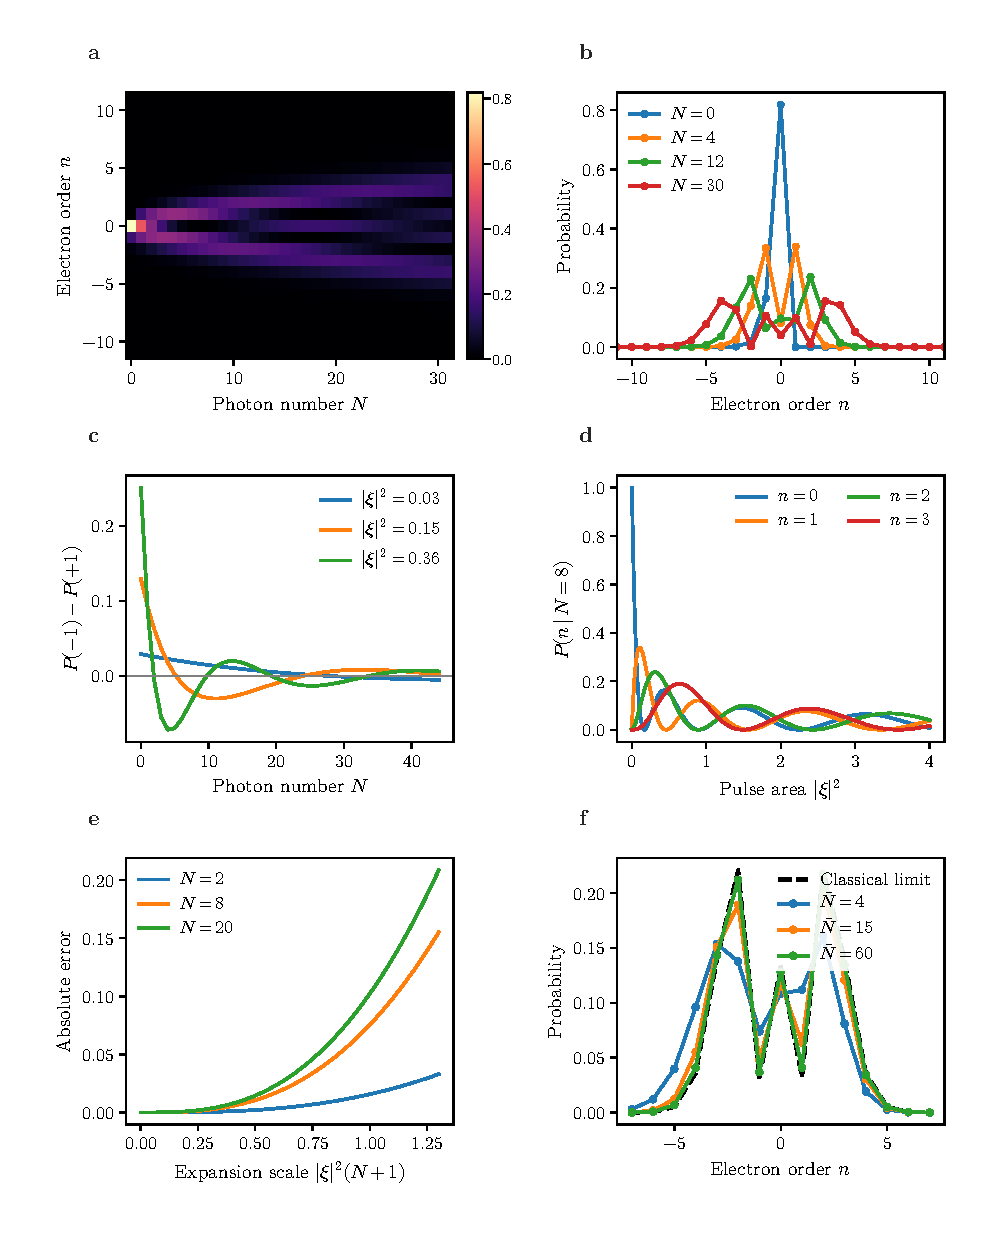
\includegraphics[width=0.96\linewidth,height=0.70\textheight,keepaspectratio]{quantum_laguerre_kernel.pdf}
\caption{\textbf{量子 PINEM 的精确数态跃迁核及其经典极限。} (a) 由\cref{eq:quantum-laguerre-amplitudes} 直接计算 $s=0.20$ 时 $N=0,\ldots,31$ 到 $n=-11,\ldots,11$ 的条件概率；黑色区包括受光子数守恒禁止的 $n>N$ 通道。(b) 同一 $s$ 下 $N=0,4,12,30$ 的电子谱：振荡结构由 Laguerre 多项式控制。(c) 三个作用强度的 $P(-1|N)-P(+1|N)$，显示真空不对称的弱耦合起点与强散射中的往返干涉。(d) 固定 $N=8$，扫描 $s\in[0,4]$，展示 $n=0,1,2,3$ 边带的精确相消零点。(e) 对 $N=2,8,20$，把二光子吸收概率与 $s^2N(N-1)/4$ 的弱耦合结果比较，横轴选用控制量 $s(N+1)$。(f) 在固定 $|\beta|=1.7$ 下取相干输入 $\bar N=4,15,60$、$|\xi|=|\beta|/\sqrt{\bar N}$，将泊松平均的精确量子核与 $J_n^2(2|\beta|)$ 比较。整图的变量均来自同一幺正演化，不附加经验展宽或拟合参数。}
\label{fig:quantum-laguerre-kernel}
\end{figure}

全部概率按\cref{eq:quantum-exact-response-kernel} 的解析系数平方计算，没有额外材料、仪器或退相干唯象参数。输入 $\xi$ 取非负实值计算概率，相位只改变振幅而不改变单个数态的边带人口；(a) 取 $s=0.20$、$N=0,\ldots,31$、$n=-11,\ldots,11$；(b) 保持 $s=0.20$，取 $N=0,4,12,30$、$n=-14,\ldots,14$；(c) 取 $N=0,\ldots,44$ 与 $s=0.03,0.15,0.36$；(d) 固定 $N=8$，在 $s\in[0,4]$ 的 440 点上画 $n=0,1,2,3$ 的概率；(e) 对 $N=2,8,20$ 扫 $\epsilon=s(N+1)\in[0.001,1.3]$ 的 140 点，纵轴为 $|P_{\rm exact}(+2|N)-s^2N(N-1)/4|$；(f) 固定 $|\beta|=1.7$、$\bar N=4,15,60$，以 $s=|\beta|^2/\bar N$ 加权 $p_N=\ee^{-\bar N}\bar N^N/N!$，对 $N\le \max\{30,\lfloor\bar N+11\sqrt{\bar N+1}\rfloor\}$ 求和，图上只显示 $n=-7,\ldots,7$。面板 (a)、(b)、(f) 展示的是有限范围内的概率，不对所示边带再次归一化；剩余概率落在未画出的阶数上。图像和数据可由 \texttt{figures/quantum\_laguerre\_kernel.py} 生成。


这些图解释了微扰理论和完整数值矩阵为何会给出不同的边带形状。微扰的控制参数不是独立的 $s$，而是入射占据数放大后的 $s(N+1)$。反演时若实际使用有限电子阶梯与有限 Fock 截断，响应矩阵的列和应接近一；一旦边界概率已不可忽略，数值重归一化会掩盖被截断的物理通道，不能当成原始精确模型的验证。

经典场替代也可以在同一个模型中受控地推出。若输入是相干态 $|\alpha\rangle$，作位移变换 $D^\dagger(\alpha)aD(\alpha)=a+\alpha$，则
\begin{align*}
D^\dagger(\alpha)U(\xi)D(\alpha)
&=\exp\!\left[(\xi\alpha^*b-\xi^*\alpha b^\dagger)
 +(\xi ba^\dagger-\xi^*b^\dagger a)\right]\\
&=\exp(\beta b^\dagger-\beta^*b)
  \exp(\xi ba^\dagger-\xi^*b^\dagger a),
\qquad \beta=-\xi^*\alpha.
\end{align*}
第二个等号用到了理想无限电子能量阶梯中 $[b,b^\dagger]=0$，以及电子平移与光子算符的对易关系；有限截断数值矩阵在边界上不具备这一性质。现在令
$|\alpha|\to\infty$、$|\xi|\to0$，同时保持 $\beta=-\xi^*\alpha$ 固定。作用在位移后的光学真空上，第二个指数产生光学激发的振幅从 $O(|\xi|)$ 开始，追踪不到光子末态的电子约化结果便趋近
\begin{equation}
\rho'_e\longrightarrow
\ee^{\beta b^\dagger-\beta^*b}\rho_e
\ee^{-\beta b^\dagger+\beta^*b}.
\label{eq:quantum-controlled-classical-limit}
\end{equation}
这才是前面经典贝塞尔边带的量子起点。单独增大 $\bar N$ 而固定 $|\xi|$，会同时增大 $|\beta|=|\xi|\sqrt{\bar N}$，比较的并不是同一个经典场作用强度。

三类状态最直接的差别体现在光子数方差。福克态满足 $\operatorname{Var}N=0$；相干态满足 $\operatorname{Var}N=\bar N$；单模热态满足 $\operatorname{Var}N=\bar N(1+\bar N)$。因为交换振幅依赖 $\sqrt N$，这些涨落会传到电子边带的宽度、尾部以及高阶矩中。

若进一步选择某个电子末态 $|m\rangle$，电子测量会对光场施加测量算符 $M_m=\langle m|U|\psi_e\rangle$。条件光场为

\begin{equation}
\rho_{\gamma|m}=\frac{M_m\rho_\gamma M_m^\dagger}{\operatorname{Tr}(M_m\rho_\gamma M_m^\dagger)}.
\label{eq:ch04-3}
\end{equation}

\cref{eq:ch04-2} 用来预测“只看电子”时的能谱；\cref{eq:ch04-3} 用来预测电子后选择后的条件光子统计。前者对应探测，后者对应条件制备。后面的数值图都从这两个问题出发。

经典 PINEM 用一个确定的复数 $\beta$ 描述光场；量子模型则保留光子数算符及其涨落。两者接近的条件不是简单“平均光子数很大”，而是光子数相对涨落和单次电子散射造成的反作用都足够小。比较有限光子数结果与大占据数极限，可以直接判断经典场替代何时成立。

把光场量子化以后，问题随即发生变化：即使平均光强相同，不同光子数涨落仍会通过产生、湮灭算符的矩阵元改变电子能谱。下面先比较这些真正可见的统计指纹。
即使平均光子数 $\bar N$ 相同，不同量子态的光子数方差和高阶矩仍可不同。由于交换振幅含有 $\sqrt N$，这些统计差异会传到电子边带的宽度、尾部和高阶矩。因而电子谱可以作为光子统计的探针，但必须选择对 $p_N$ 足够敏感、又不容易被有限分辨率抹平的观测量。

\begin{figure}[!htbp]
\centering
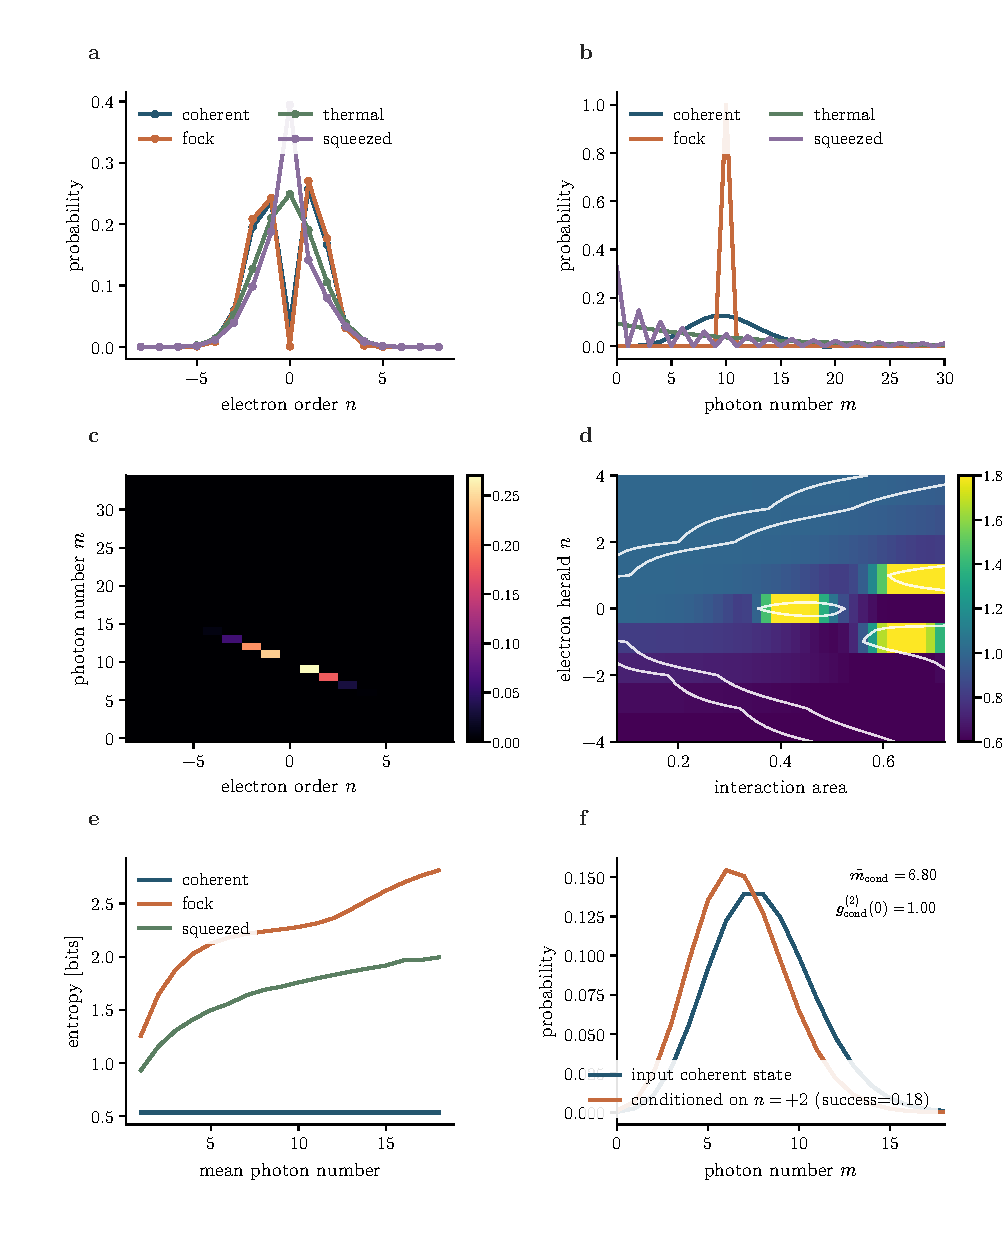
\includegraphics[width=0.96\linewidth,height=0.70\textheight,keepaspectratio]{quantum_light_fingerprints.pdf}
\caption{\textbf{相同平均光子数为何仍产生不同电子谱}\quad 计算保持平均光子数和相互作用参数不变，只改变入射光场的光子数分布。第一排先把“同一平均值、不同涨落”讲清楚：相干态、福克态、热态和压缩态对应不同的光子数分布，因此电子边带也呈现不同的宽度、尖锐度和尾部。右上角的联合概率图进一步说明，电子能量与剩余光子数之间存在清晰的相关梯形结构。第二排则进入真正的量子指纹：电子后选择后的条件 Fano 因子图显示测量会把原本近经典的光场推向次泊松或超泊松区域；电子--光子纠缠熵曲线给出“信息究竟留在电子上还是转入联合态”的预算；最右侧的条件光子数分布则直接展示测量回作用怎样重塑光场本身。}
\label{fig:ch04-novel-extensions--23-quantum-light-fingerprints}
\end{figure}

数值实现中，电子阶梯平移与单模光子产生、湮灭共同决定联合分布：
\[U(\xi)=\exp(\xi a^\dagger b-\xi^*b^\dagger a),\quad P_{nm}=|\langle n,m|U|0,\psi_\gamma\rangle|^2,\quad P_n=\sum_mP_{nm}.\]
输入相干态、光子数态和压缩真空是纯态；热光输入需要对各光子数分量做密度算符平均，不可将其视为具有固定波函数的纯联合态。四种入射光态的基线均值为 $\bar N=10$，耦合脉冲面积 $|\xi|=0.38$，电子阶数范围 $|n|\le8$，光子 Fock 截断 $m\le34$；压缩真空参数选为 $r=\operatorname{arsinh}\sqrt{10}$，以确保与其他输入具有相同的真实平均光子数。后选择部分单独使用下文所列参数，不将其当成基线的同一数值实验。


\begin{figure}[!htbp]
\centering
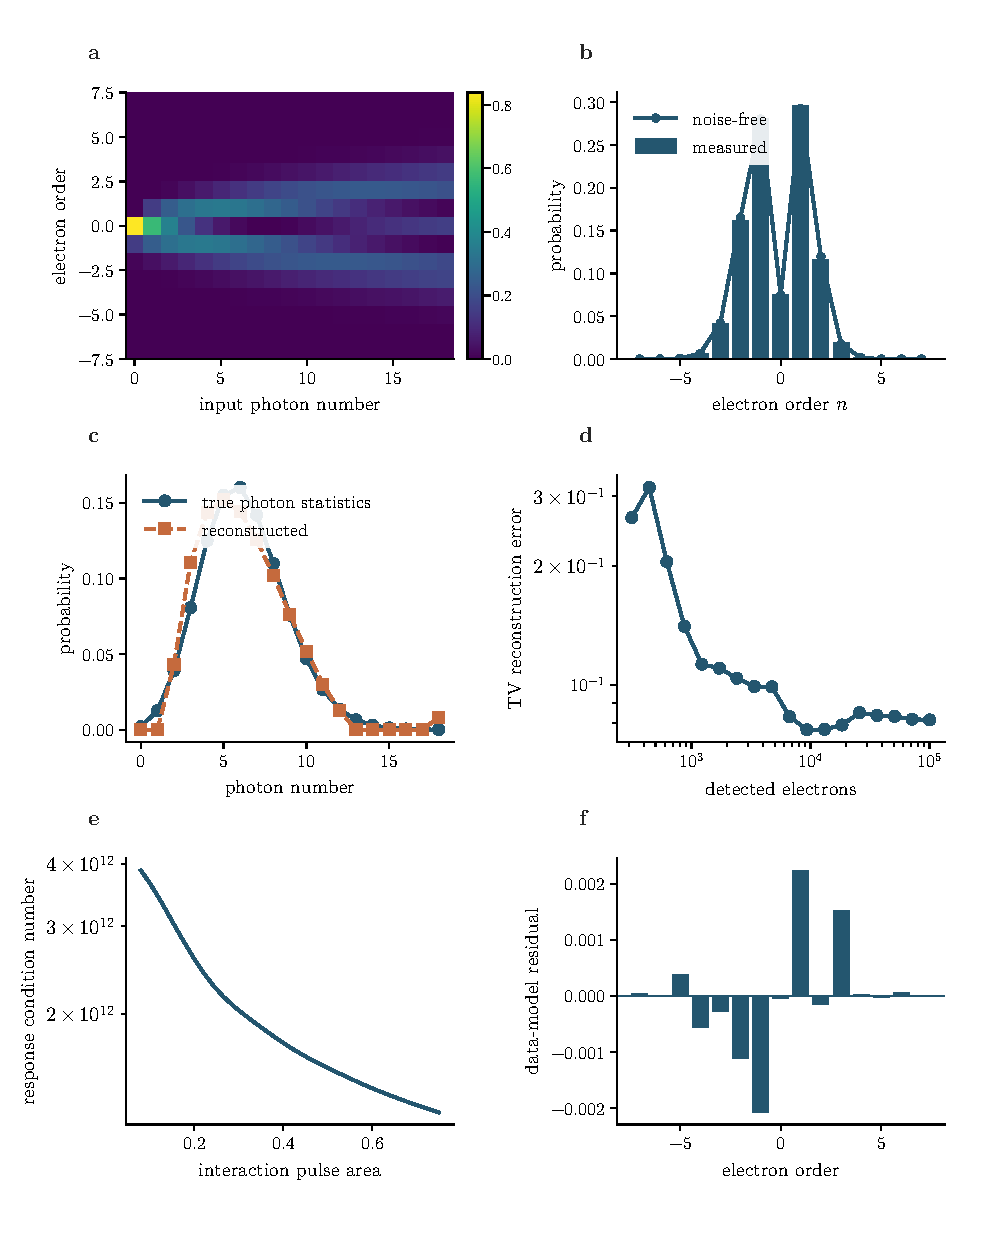
\includegraphics[width=0.96\linewidth,height=0.70\textheight,keepaspectratio]{photon_statistics_tomography.pdf}
\caption{\textbf{由电子谱反演光子数分布}\quad 先用数态输入逐列计算响应矩阵 $K_{nN}=P(n\mid N)$。未知光子数分布 $p_N$ 产生的电子谱满足 $q_n=\sum_NK_{nN}p_N$。图中先展示响应矩阵和带计数噪声的电子谱，再用非负吉洪诺夫（Tikhonov）正则化反演 $p_N$。 计数增加时重构误差下降；相互作用过弱或过强时，响应矩阵不同列变得难以区分，条件数升高。因此“能测到边带”并不等于“能稳定反演光子统计”。}
\label{fig:ch04-novel-extensions--25-photon-statistics-tomography}
\end{figure}

数值实现中，先由每个数态输入计算响应矩阵 $K_{nN}=P(n|N)$，再求解带非负约束的正则化反问题：
\[q_n=\sum_NK_{nN}p_N,\quad \widehat{\mathbf z}=\arg\min_{\mathbf z\ge0}\bigl\|K\mathbf z-\mathbf q\bigr\|_2^2+\lambda\bigl\|\mathbf z\bigr\|_2^2,\quad \widehat p_N=\frac{\widehat z_N}{\sum_M\widehat z_M}.\]
设输入为截断归一的 Poisson 分布 $p_N\propto e^{-6.2}6.2^N/N!$、$N=0,\dots,18$；$n_e=7$、$n_\gamma=30$、$|\xi|=0.42$，泊松计数 $N_e=18000$、随机种子 4、$\lambda=10^{-3}$。电子计数扫描 $10^{2.5}\!\sim 10^5$（18 点，种子 3）；相互作用面积扫描 $[0.08,0.75]$（30 点）。响应矩阵最大与最小奇异值之比（最小值按 $10^{-12}$ 截断）用于定义数值条件数，误差定义为总变差距离 $D_{\mathrm{TV}}=\tfrac12\sum_N|\widehat p_N-p_N|$；(f) 所画 $y-K\widehat p$ 是\emph{正向拟合残差}，不是采样得到的贝叶斯后验预测分布。数值实现先在堆叠矩阵 $[K;\sqrt\lambda I]$ 上调用非负最小二乘求得 $\widehat{\boldsymbol z}$，随后统一归一化；并非在优化器内部施加归一化等式约束。

具体到各面板，(a) 逐一制备 $N=0,\dots,18$ 的数态，按同一联合哈密顿量计算响应矩阵：\[K_{nN}=\sum_m\left|\langle n,m|\exp(-\ii\,0.42H_{\rm int})|0,N\rangle\right|^2.\] (b) 比较 $p=Kp_N$ 与 $N_e=18000$ 次多项抽样 $y=c/N_e$（种子 4）；(c) 画 $p_N\propto e^{-6.2}6.2^N/N!$ 及 NNLS + $10^{-3}$ 正则后的 $\widehat p_N$；(d) 逐个样本数 $N_e=\lfloor10^{2.5}\rfloor$--$10^5$，种子固定 3，取 $\tfrac12\sum|\widehat p-p|$；(e) 扫 $\xi=0.08$--$0.75$（30 点）绘 $\kappa_2(K)=s_{\max}/\max(s_{\min},10^{-12})$；(f) 画 $y-K\widehat p$，是拟合残差而非贝叶斯后验预测。采用 $|n|\le7,m\le30$，输入光子数上限 18。


然而，只测电子的谱还不能反映全部联合态。沿着这一差别继续走下去，就自然需要讨论电子--光子纠缠、偏迹和后选择。\textsuperscript{\hyperref[ch04-ref3]{[3]}}
联合演化后，电子能量与光子数通常不能写成两个独立态的乘积。若忽略光场，这种纠缠表现为电子约化态的混合；若对电子末态做条件选择，同一关联又可以被利用来制备条件光场。联合概率、约化纯度和条件光子统计分别给出这一关联的三个可观测侧面。

量子 PINEM 的早期理论首先告诉我们，电子谱可以读取光子统计，电子后选择也可以反过来改变光场。但到这里仍有一个实验上更严格的问题：条件光场是否真的表现出不能由经典随机场解释的统计？2025 年 Arend 等把能量分辨单电子探测与光子的 Hanbury Brown--Twiss 符合测量结合起来，在集成波导中直接测量电子能量损失与产生光子数的关联。选择单量子电子能损事件后，条件光场表现出单光子反聚束；选择双量子能损事件则增强双光子符合。\textsuperscript{\hyperref[ch04-ref5]{[5]}}

这类实验要求把\cref{eq:ch04-3} 从“形式上的条件态”变成一个完整的测量链。若电子结果记为 $m$，光子探测结果记为 $k$，真正比较的是联合概率
\begin{equation}
P(m,k)=\operatorname{Tr}\!\left[(\Pi_m^{(e)}\otimes\Pi_k^{(\gamma)})\,U(\rho_e\otimes\rho_\gamma)U^\dagger\right],
\label{eq:ch04-joint-measurement}
\end{equation}
以及条件相关函数 $g^{(2)}(0|m)$。电子能量损失与光子数相关并不自动等于非经典光；只有在条件统计中出现经典场不能给出的反聚束或其他非经典判据时，才完成从“相关”到“非经典条件态”的证据升级。

这也修正了一个容易产生的研究误区。提高电子--光子耦合并不只是为了让边带更多。强耦合真正有价值的地方，是它增加了联合态中可访问的光子数范围，使电子测量算符 $M_m$ 可以对光场实施更丰富的非高斯条件操作。2026 年自由电子量子光学综述已经把条件光子制备、量子门、纠错原语和量子计量列为同一联合散射框架下的不同任务。\textsuperscript{\hyperref[ch04-ref6]{[6]}} 因而以后设计“新量子光态”时，应同时报告三件事：条件态的非经典指标、成功概率，以及在损耗和有限电子能量分辨率下这些指标还能保留多少。

单频相互作用中的电子后选择只要求记录一个能量阶数。若同时存在 $\omega$ 和 $2\omega$ 的两个独立量子光模式，且它们分别携带确定的方位角动量 $\ell_1\hbar$ 与 $\ell_2\hbar$，电子散射的末态还可以按照能量阶 $N$ 和角动量阶 $L$ 共同标记。设两个光场模式的联合初态为 $\rho_{\gamma}$，总幺正算符 $U$ 在电子--双模光场 Hilbert 空间上作用，则归一化之前的条件光场态由
\begin{equation}
M_{NL}={}_e\!\langle N,L|U|0,0\rangle_e,\qquad
\widetilde\rho_{\gamma|NL}=M_{NL}\rho_{\gamma}M_{NL}^\dagger,
\label{eq:two-mode-optical-kraus}
\end{equation}
确定。测量结果的成功概率是 $p_{NL}=\operatorname{Tr}\widetilde\rho_{\gamma|NL}$，只在 $p_{NL}>0$ 时才将其除以 $p_{NL}$ 得到条件态。无论采用哪一种具体相互作用模型，完备电子测量满足 $\sum_{NL}M_{NL}^\dagger M_{NL}=\mathbb I_{\gamma}$；若探测器有遗漏通道，该等式必须把未记录结果也包括进去。

在只允许交换上述两种基本光量子的最小模型中，通道标签服从 $N=n_1+2n_2$ 与 $L=n_1\ell_1+n_2\ell_2$。两个方程的系数矩阵行列式为 $\ell_2-2\ell_1$。当行列式非零时，指定 $N,L$ 至多选择一组整数交换次数；当行列式为零时，多个路径可能在同一电子末态相干汇合。但路径合并本身并不保证条件光场具有负性或纠缠：还必须从 $M_{NL}\rho_{\gamma}M_{NL}^\dagger$ 计算光子数统计、条件成功率和相应非经典性判据。这样，合成维度章节的二维合成路径读出才真正成为量子光态制备的一个测量操作，而非仅仅是多了一条作图坐标。

\textsuperscript{\hyperref[ch04-ref7]{[7]}}
前面的量子 PINEM 都围绕光子产生和湮灭：电子能量改变，光子数也改变。2026 年 Zheng 与 Kfir 强调了另一类容易被忽略的量子作用。电子即使没有发生净光子交换，也可以给腔模施加可测相位回踢；反过来，光场也给电子积累色散相位。这个过程可以写成电子--光子之间的色散耦合，并被用于讨论不改变电子量子态的电子计数和亚散粒噪声测量。

为了看清它与\cref{eq:ch04-1} 的差别，可以先写一个最小有效模型。令 $\hat N_e$ 表示与该光学模式发生作用的电子数或电子路径占据，$\hat n_\gamma=a^\dagger a$ 为光子数，则弹性色散作用具有
\begin{equation}
U_{\rm el}=\exp\!\left(\ii\chi\,\hat N_e\hat n_\gamma\right)
\label{eq:ch04-elastic-unitary}
\end{equation}
这样的结构，其中 $\chi$ 是单电子造成的模式相位。若恰有一个电子通过，光子数本身不变，但相干态满足
\begin{equation}
U_{\rm el}|1\rangle_e|\alpha\rangle_\gamma
=|1\rangle_e|\alpha \ee^{\ii\chi}\rangle_\gamma.
\label{eq:ch04-phase-kickback}
\end{equation}
因此“没有能量损失峰”并不等于“电子没有对光场做任何事”。这里被写入的是相位，而不是光子数。

若电子处于两条路径的叠加，而且只有其中一路与腔模显著耦合，\cref{eq:ch04-elastic-unitary} 会把电子路径与光场相位关联起来。若光场相位最终被读出，就可以获得电子是否经过作用区的信息；若光场不被读出，则同一哪一路信息会降低电子路径相干性。这个例子把量子光章节和开放系统章节连了起来：量子测量、回作用和退相干并不是三件互不相干的事，而是对同一个联合幺正演化选择不同偏迹或条件测量后的结果。

弹性作用与非弹性 PINEM 也不能在所有情况下简单相加。因为
\begin{equation}
[\hat n_\gamma,a]=-a,
\end{equation}
所以色散相位会旋转后续的产生、湮灭算符。若实验同时具有显著的弹性相位回踢和光子交换，正确问题应是两个联合算符的有序乘积，而不是把“相位偏移”和“边带概率”分别拟合后再相加。这个非对易性在通常强经典场 PINEM 中很容易被吸收到参考相位里，但在少光子、电子路径叠加或重复作用的量子协议中可能成为可测资源。能否观测到次序效应，需要在同一场模式与探测设置下比较两种作用顺序的完整计数分布。


\textsuperscript{\hyperref[ch04-ref8]{[8]}}
\section{相位测量}
电子能谱测量把 $|\psi_e\rangle=\sum_n c_n|E_0+n\hbar\Omega\rangle$ 投影到能量本征态，因此直接得到 $|c_n|^2$，却破坏了不同能量阶之间的相位。对真正的自由电子量子信息任务，这不是一个小技术问题：如果实验永远只能在能量基测量，就无法像普通量子比特那样自由选择互补测量基。Zou 等在 2026 年提出利用 PINEM 与辅助量子光，把能量基的 Fourier 共轭 comb basis 变成非破坏投影测量。该工作目前是预印本方案，因此本节把它作为“测量理论接口”而不是已完成实验。

沿用量子 PINEM 的能量平移算符
\begin{equation}
b_\Omega|E\rangle=|E-\hbar\Omega\rangle,
\qquad b_\Omega^\dagger b_\Omega=1,
\label{eq:ch04-comb-shift}
\end{equation}
定义广义 comb 态
\begin{equation}
|\mathrm{comb}(\phi)\rangle
\propto\sum_{k\in\ZZ}\ee^{-\ii k\phi}|E-k\hbar\Omega\rangle,
\qquad \phi\in[-\pi,\pi).
\label{eq:ch04-comb-state}
\end{equation}
它是平移算符的本征态：
\begin{equation}
b_\Omega|\mathrm{comb}(\phi)\rangle=\ee^{\ii\phi}|\mathrm{comb}(\phi)\rangle.
\label{eq:ch04-comb-eigen}
\end{equation}
因此能量阶数 $k$ 与 comb 相位 $\phi$ 是离散 Fourier 共轭变量。能量测量问“电子在哪个能量格点”，comb 测量问“相邻能量格点之间共同的平移相位是什么”。这正是为什么两种测量能够提供互补信息。

量子 PINEM 幺正算符写成
\begin{equation}
U(g)=\exp\!\left(g a^\dagger b_\Omega-g^*b_\Omega^\dagger a\right).
\label{eq:ch04-comb-unitary}
\end{equation}
如果电子恰处在 $|\mathrm{comb}(\phi)\rangle$，利用\cref{eq:ch04-comb-eigen}，电子算符可以在该本征子空间中替换为相位因子，于是
\begin{equation}
U(g)|\mathrm{comb}(\phi)\rangle|\psi_\gamma\rangle
=|\mathrm{comb}(\phi)\rangle
D\!\left(ge^{\ii\phi}\right)|\psi_\gamma\rangle,
\label{eq:ch04-comb-displacement}
\end{equation}
其中 $D(\alpha)=\exp(\alpha a^\dagger-\alpha^*a)$。该式表明，电子 comb 相位 $\phi$ 控制辅助光场位移 $ge^{\ii\phi}$ 的相空间方向。于是无需吸收电子或测量其能量，只要对辅助光做同相与正交分量的 homodyne，就可以反推出 $\phi$。

理想情况下，用两个正交压缩方向的辅助模式分别读取 $\cos\phi$ 与 $\sin\phi$。若两个实耦合为 $g_1,g_2$，homodyne 均值满足量级关系
\begin{equation}
X_1\sim g_1\cos\phi,\qquad P_2\sim g_2\sin\phi,
\label{eq:ch04-comb-quadrature}
\end{equation}
因此，只有在两路读出提供独立且充分校准的正交信息时，才能从测得的二维位移估计 $\phi$。有限压缩使这些均值带噪，原文给出的可分辨相位尺度随 $1/(|g|e^r)$ 缩小，其中 $r$ 是压缩参数。这个标度清楚地告诉我们实验资源如何进入测量精度：不是“压缩越大越量子”这种泛泛说法，而是辅助光相空间噪声越窄，越能区分相邻 comb 相位。

更深的一点是，这个测量把“电子相位”转移到光学辅助系统后再测，因此电子本身可以保留在能量梳叠加中。Zou 等据此讨论了自由传播二次相位误差的稳定子检测和 EPR steering。对本书而言，更重要的结论是：从这一刻起，电子测量不必等同于 EELS。能量基、comb 基以及它们之间的可编程中间基，可以像普通量子信息中的测量轴一样成为实验设计变量。

量子 PINEM 文献很早就预测电子--光子纠缠，但“联合态在理论上不可分”与“实验直接验证纠缠”是两个证据等级。Henke 等 2025 年的预印本报告了自由电子路径与所产生光子偏振之间的纠缠：电子先被制备成两路径叠加，经过纳米结构产生跃迁辐射，光子偏振与电子路径相关；随后通过联合量子态层析重构电子--光子密度矩阵，并报告 Peres--Horodecki 可分性判据超过七个标准差的违反。2026 年 Quantum 2.0 会议论文又以同一实验方向报告了该验证。\textsuperscript{\hyperref[ch04-ref9]{[9]}\hyperref[ch04-ref10]{[10]}}

这一实验不是标准的 PINEM 吸收--受激发射几何，而是自由电子路径与跃迁辐射偏振的混合纠缠，因此不能拿它来声称“PINEM 中已经实验观察到任意强电子--光子纠缠”。它真正改变的是证据基线：自由传播电子和单光子之间的纠缠已经不再只是理论可能性。今后任何基于 PINEM、腔模或极化激元的纠缠方案，都应把目标从“产生非可分联合波函数”升级为“给出可实施的互补测量和纠缠见证”。

对二比特型路径--偏振子空间，最简单的层析语言是
\begin{equation}
\rho_{e\gamma}=\frac14\sum_{\mu,\nu=0}^{3}
T_{\mu\nu}\,\sigma_\mu^{(e)}\otimes\sigma_\nu^{(\gamma)},
\qquad
T_{\mu\nu}=\langle\sigma_\mu\otimes\sigma_\nu\rangle.
\label{eq:ch04-twoqubit-tomo}
\end{equation}
只测电子能量或只测光子数都不足以恢复这些相关张量。必须改变双方测量基，才能区分经典相关与相干叠加。comb-basis 方案的意义也因此更清楚：它提供了一种可能的电子互补测量轴，使能量--相位型电子--光子纠缠未来有机会像路径--偏振纠缠一样被完整验证。


理想 comb 态是相位表示中很便利的广义本征态，但真实电子的能谱总有有限宽度。这里应先问一个比“能不能测 comb 相位”更具体的问题：假设电子只占据有限个能量阶，辅助光读出究竟还能区分多细的相位？当有限能量带宽与有限光学测量噪声同时存在时，二者不能由一个任意的“测量精度”参数替代。

令电子只在 $M=2K+1$ 个相邻能量阶中有非零振幅。最直接的受限 comb 态是
\begin{equation}
|\phi;M\rangle=\frac{1}{\sqrt M}\sum_{n=-K}^{K}\ee^{-\ii n\phi}|n\rangle,
\qquad \langle\phi;M|\phi;M\rangle=1.
\label{eq:ch04-finite-comb}
\end{equation}
对这一有限态，能量平移算符不再具有精确相位本征值，因为最外两阶会被移出截断子空间。在标准的周期相位 POVM 中，测得相位 $\vartheta$ 的概率密度为
\begin{equation}
p_M(\vartheta|\phi)=\frac{1}{2\pi M}
\left|\sum_{n=-K}^K \ee^{\ii n(\vartheta-\phi)}\right|^2
=\frac{1}{2\pi M}\frac{\sin^2[M(\vartheta-\phi)/2]}{\sin^2[(\vartheta-\phi)/2]},
\label{eq:ch04-fejer}
\end{equation}
分母为零处按连续极限取值。它并不是人为选取的高斯窗口，而是有限能量梳的 Fourier 核。主峰随 $M$ 增大而变窄，却始终具有旁瓣；因此把有限带宽实验的相位响应完全视作正态分布，在远离工作点的置信区间可能出错。相位是周期变量，还必须使用圆周误差而不是未经展开的直线差值。

另一方面，如果电子以理想 comb 相位控制辅助光位移，光学读出仍会有独立的噪声。为明确区分量子协议与仪器模型，下面只建立一个\textbf{有效双正交指针基准}：两路已校准光学正交量的均值取
\begin{equation}
\boldsymbol\mu(\phi)=g(\cos\phi,\sin\phi),\qquad
\boldsymbol Y=\boldsymbol\mu(\phi)+\boldsymbol\epsilon,
\quad\epsilon_X,\epsilon_P\overset{\rm iid}{\sim}{\cal N}(0,\sigma^2),
\label{eq:ch04-pointer}
\end{equation}
其中 $g$ 是可观测指针位移半径，不与前面的散射哈密顿量参数强行等同；单个测量通道的有效噪声方差假设为
\begin{equation}
\sigma^2=\frac{e^{-2r}}4+\sigma_{\rm det}^2.
\label{eq:ch04-pointer-noise}
\end{equation}
这里 $X=(a+a^\dagger)/2$ 的真空方差为 $1/4$；$r$ 是该被测正交量的有效压缩参数，$\sigma_{\rm det}$ 是附加电子无关读出噪声。把两路都视为独立同方差信道，意味着采用了两只分别准备和测量的辅助模式，
\emph{并不}表示一个单模上可以无代价同时测量非对易的 $X$ 与 $P$。这项近似使电子--光学读出的资源预算可以直接估算，但不代表已求解了完整的电子--双模联合散射。两路输出的均值沿相空间半径为 $g$ 的圆周运动；只测单路 $X$ 会有 $\phi$ 与 $-\phi$ 的全局歧义，同时测两路才可局域解开它。

由二维正态似然，单事件经典 Fisher 信息为
\begin{equation}
F_{\phi\phi}^{(1)}=
(\partial_\phi\boldsymbol\mu)^\mathsf T
(\sigma^2 I_2)^{-1}(\partial_\phi\boldsymbol\mu)
=\frac{g^2}{\sigma^2}.
\label{eq:ch04-pointer-fisher}
\end{equation}
$N_e$ 次独立接受事件的信息为 $N_eF_{\phi\phi}^{(1)}$，局域无偏估计的 Cramér--Rao 界是 $\Delta\phi\ge\sigma/(g\sqrt{N_e})$。此处的测量成功率不包括在“每接受事件”的信息中：若每入射电子仅有概率 $\eta_{\rm acc}$ 进入可用的条件样本，则每入射电子的信息预算应该再乘 $\eta_{\rm acc}$。并且当 $\sigma_{\rm det}$ 有非零底线时，任意提高 $r$ 都不能无限提升 $F_{\phi\phi}$。

\begin{figure}[!htbp]
\centering
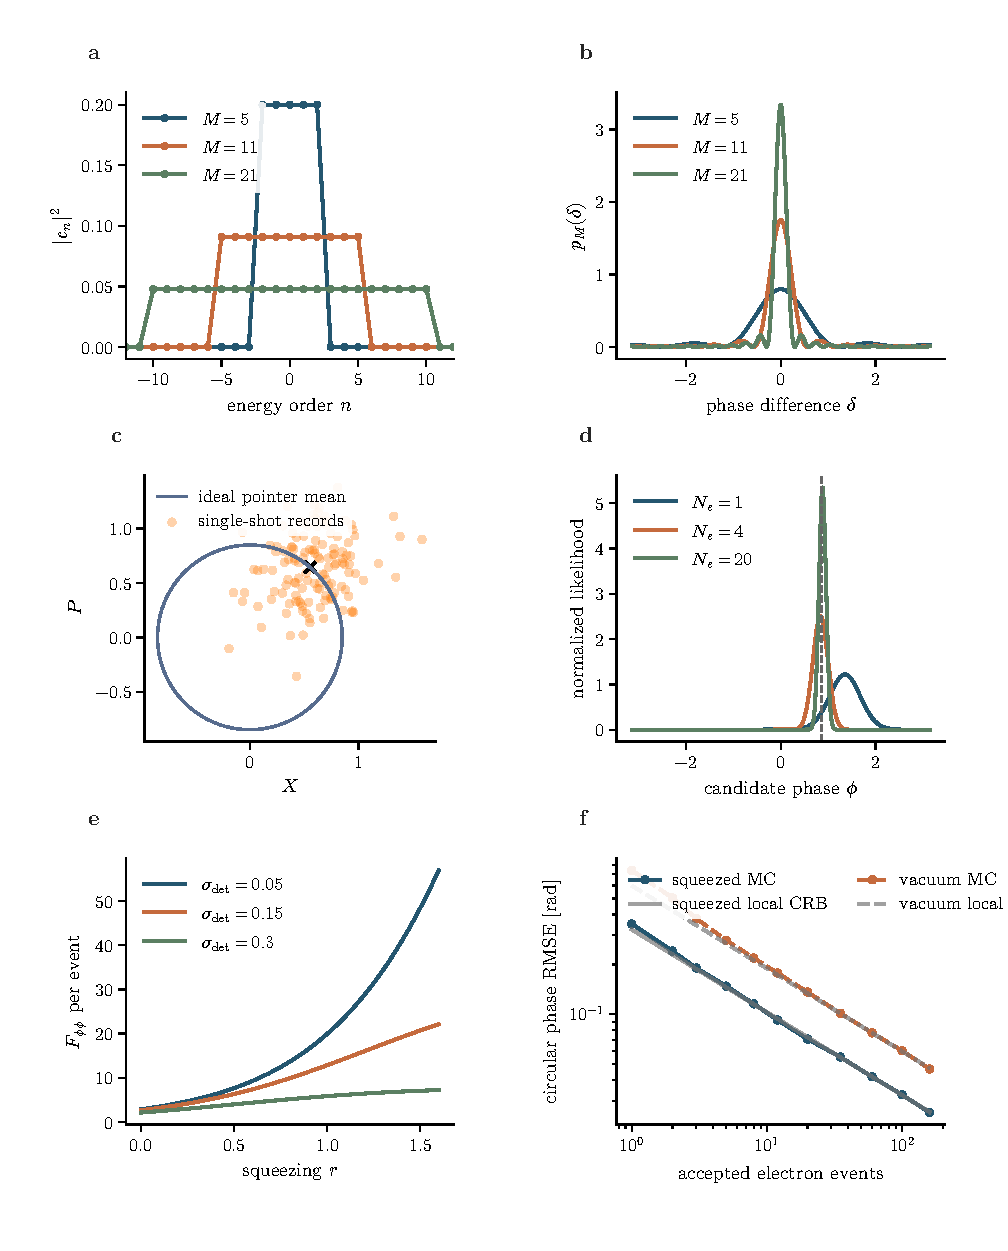
\includegraphics[width=0.97\linewidth,height=0.70\textheight,keepaspectratio]{comb_measurement.pdf}
\caption{\textbf{从有限 comb 相位态到有噪声的光学指针读出}\quad (a) 不同有限能量梳的能量人口；(b) 相应的周期相位 POVM 响应由有限 Fourier 核直接生成，带宽越大，主峰越窄；(c) 理想指针均值在两路正交量相空间中沿圆周运动，实际单次读数构成二维随机云；(d) 独立接受更多电子事件时的周期相位似然；(e) 有附加仪器噪声时，压缩带来的单事件相位 Fisher 增益必然饱和；(f) 角度最大似然估计的 Monte Carlo 圆周均方误差与局域 Fisher 下界。前三幅解释有限态和指针机制，后三幅解释可实现精度的统计限制，不把条件概率和成功率混为一谈。}
\label{fig:ch04-comb-measurement}
\end{figure}

具体到各面板，(a) 在 $n=-12,\ldots,12$ 上显示 $M=5,11,21$ 的有限均匀 comb，非零人口皆为 $1/M$；(b) 将同样三个 $M$ 代入\cref{eq:ch04-fejer}，角度网格 $\delta\in[-\pi,\pi]$ 共 700 点，密度对圆周积分为 1。(c) 取真相位 $\phi_0=0.86$、指针半径 $g=0.85$、压缩参数 $r=0.65$、附加高斯噪声标准差 $\sigma_{\rm det}=0.09$，于是 $\sigma^2=e^{-2r}/4+\sigma_{\rm det}^2\simeq0.07623$；绘制 130 个独立二维读数。(d) 固定前述伪随机序列（种子 1609），依次用前 $N_e=1,4,20$ 个样本求 $\log L(\phi)=-\sum_j\|\boldsymbol Y_j-\boldsymbol\mu(\phi)\|^2/(2\sigma^2)$，减去最大值再指数化，利用梯形法对 $[-\pi,\pi]$ 积分归一化。(e) 固定 $g=0.85$，扫描 $r\in[0,1.6]$ 共 120 点，比较 $\sigma_{\rm det}=0.05,0.15,0.30$，按\cref{eq:ch04-pointer-fisher} 计算每接受事件 Fisher 信息。(f) 对 $N_e=1,2,3,5,8,12,20,35,60,100,160$ 分别统计 2300 组独立采样，比较 $r=0.65$ 与 $r=0$；每组以 $\operatorname{atan2}(\sum P_j,\sum X_j)$ 估计相位，再以 $\arg \ee^{\ii(\widehat\phi-\phi_0)}$ 定义圆周误差。灰色界线为 $\sigma/(g\sqrt{N_e})$，仅代表局域大样本极限；它不吸收有限 comb 的相位旁瓣，也不计后选择成功率。整图没有添加未声明的实验效率常数。


这张图也给出了设计电子互补测量的清晰顺序。先用有限电子带宽计算态制备本身的相位核，排除小 $M$ 带来的分辨率限制；再依据辅助光的实际压缩、损耗和探测噪声计算读出核；最后把成功率并入每入射电子的信息指标，而不是只报告被选择出的少量事件可以达到多小的统计误差。实际实验若具有显著非高斯测量噪声，还必须重新计算完整似然，不能继续使用这里的高斯指针界。

经典极限应由无量纲比值判断。需要比较光子数相对涨落、电子一次交换的能量与场总能量之比，以及探测器是否仍能分辨不同光子数对应的动力学。只有这些量都变小，量子模型才稳定地收敛到经典相位调制模型。

\begin{figure}[!htbp]
\centering
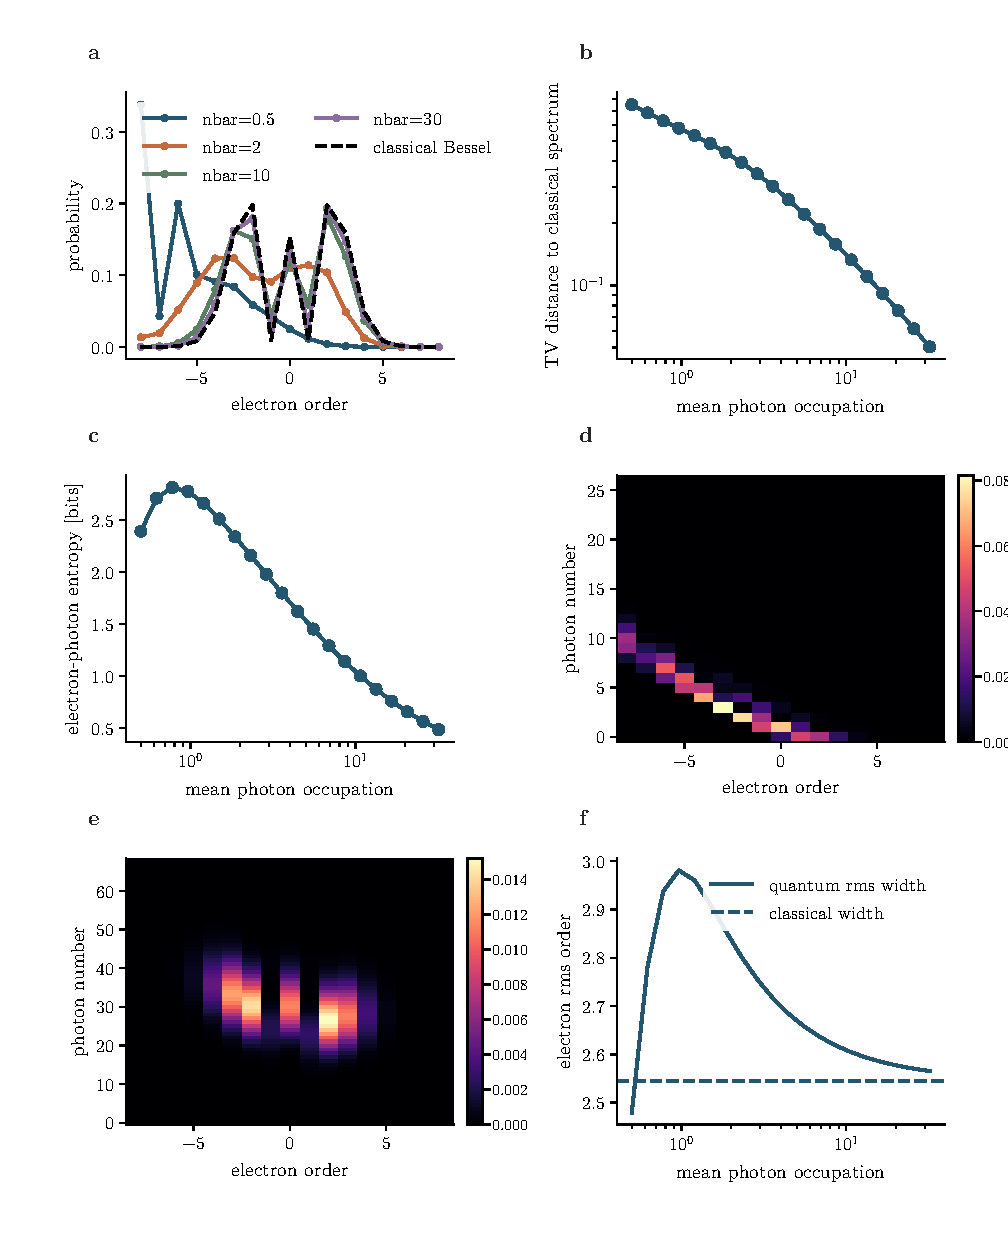
\includegraphics[width=0.96\linewidth,height=0.70\textheight,keepaspectratio]{quantum_to_classical_crossover.pdf}
\caption{\textbf{保持经典耦合不变时的量子—经典极限}\quad 为了只考察量子涨落而不改变经典 PINEM 强度，计算保持 $\beta=1.8$ 不变，并令量子相互作用面积随平均光子数按 $|\xi|=|\beta|/\sqrt{\bar N}$ 缩放。随着 $\bar N$ 增大，相干态的相对光子数涨落减小，电子边带逐渐逼近经典贝塞尔分布。 图中用总变差距离定量表示两种电子谱的差别，同时跟踪电子—光子纠缠熵和电子均方根阶数。若这些量同时收敛，才可以把大占据数称为经典场极限。}
\label{fig:ch04-novel-extensions--30-quantum-to-classical-crossover}
\end{figure}

为隔离相对光子数涨落，固定经典耦合而缩放量子相互作用：
\[|\beta|=1.8,\qquad |\xi|=\frac{|\beta|}{\sqrt{\bar N}},\qquad P_n^{\rm cl}=\frac{J_n^2(2|\beta|)}{\sum_{|m|\le n_e}J_m^2(2|\beta|)},\qquad D_{\rm TV}=\frac12\sum_n|P_n^{\rm q}-P_n^{\rm cl}|.\]
取 $\bar N\in[0.5,32]$（20 个对数点），能级截断 $n_e=8$，光子数截断随均值取 $n_\gamma=\max\{26,\lfloor\bar N+5.5\sqrt{\bar N}+8\rfloor\}$。图中的谱截面取 $\bar N=0.5,2,10,30$，联合态图取 $\bar N=1,30$；纠缠熵与能谱 RMS 宽度由同一截断联合态计算。

具体到各面板，(a) 在 $\bar N=0.5,2,10,30$ 比较量子 $P_n^{\rm q}$ 与有限截断归一的 $J_n^2(3.6)$；(b) 对 $\bar N\in[0.5,32]$ 的 20 个对数点计算 $D_{\rm TV}$；(c) 同一\emph{纯联合态}求电子约化熵；(d,e) 分别画 $\bar N=1$ 与 30 的 $P_{nm}$；(f) 取 $\sigma_n=\sqrt{\sum(n-\bar n)^2P_n}$ 与经典常值比较。每次均取 $|\xi|=1.8/\sqrt{\bar N}$、$|n|\le8$、$m_{\max}=\max\{26,\lfloor\bar N+5.5\sqrt{\bar N}+8\rfloor\}$，截断态在计算后归一，故大 $\bar N$ 不等同于连续光子数的精确极限。


取平均光子数都为 $\bar N$ 的三种光场。福克态固定在 $N=\bar N$；相干态的光子数服从 泊松分布；热态服从几何分布。三者的一阶矩相同，但方差分别为


\begin{equation*}
0,\qquad \bar N,\qquad \bar N(1+\bar N).
\end{equation*}


相互作用矩阵元含有 $\sqrt N$。因此即使只看一次吸收过程，平均跃迁强度涉及 $\langle N\rangle$；一旦比较更高阶过程或涨落，$\langle N^2\rangle$ 也会进入，而 $\langle N^2\rangle=\bar N^2+\operatorname{Var}(N)$。所以三种光场从二阶统计开始必然分开。

这给出了读图时最简单的判断：若某个电子观测量只依赖 $\bar N$，三种曲线应重合；若曲线分开，说明该观测量已经读取到光子数涨落或更高阶矩。后面的统计指纹图正是用这一标准比较不同光场，而不是只比较平均强度。

耦合太弱时，各种光子态都主要停留在零阶边带，电子谱几乎没有区分能力；耦合太强而分辨率有限时，过多边带又会被仪器平均。连续扫描平均光子数、损耗和耦合强度，可以找到光子统计最容易被识别的中间区域。


二阶相关 $g^{(2)}$、法诺（Fano）因子、$\sqrt N$ 依赖的交换频率、条件态和层析分别探测光子统计的不同信息。任意一个单独的电子谱量都不能完整恢复一般量子光场，所以不同观测必须通过同一个电子—光场前向模型联合解释。


\medskip
光子数分布先决定条件散射振幅，电子测量再把这些振幅压缩成可观测计数。把统计量、条件测量和反演放在一起，可以看出哪些信息已经进入电子边带，哪些信息仍留在电子—光子关联中。


\medskip
量子 PINEM 的最小描述必须先演化电子--光场联合态，再根据实验读出对未测量自由度取偏迹；因此平均光子数相同并不保证电子谱相同。

光子数分布通过 $\sqrt N$ 矩阵元进入散射振幅，福克态、相干态和热态的方差与高阶矩因而能够留下不同的电子谱指纹。

电子后选择对应测量算符 $M_m$，可以改变条件光场的统计与非经典性；但更强的条件效应通常伴随更低成功概率，必须同时报告两者。

Kfir 2019、Di Giulio--García de Abajo 2020 与 Baranes 等 2022 分别支撑强耦合电子--光子纠缠、量子光整形自由电子以及电子诱导光子纠缠的理论背景；Zheng--Kfir 2026 又说明即使没有净光子交换，弹性色散相位仍会产生量子回作用。

量子化联合态告诉我们信息如何在电子与光子之间重新分配；实验若只观测其中一部分，就必须把其余自由度迹掉，这会自然引出开放系统动力学。

\clearpage
\par\medskip 本章的六联图采用有限光子 Fock 截断，不能把所有面板都解释为相同的 $\bar N$ 扫描。基线的四种输入态把均值匹配到 $\bar N=10$，但当单独扫描压缩参数 $r$ 时，压缩真空的均值随 $\sinh^2r$ 改变。反演章节只把光子数\emph{对角分布}作为未知量；若光场有待重建的数态相干，单套电子能量人口响应矩阵并不足以恢复完整光学密度矩阵。


\noindent \figref{fig:ch04-novel-extensions--23-quantum-light-fingerprints}：六面板计算逐项核对。\par\noindent
(a) 对平均光子数均为 $10$ 的相干态、$|10\rangle$、热光态与压缩真空计算电子边带概率 $P_n$，共同使用 $|n|\le8,m\le34,|\xi|=0.38$；(b) 对相同四类\emph{入射}光态画其原始光子数分布 $p_m$，截断 $m=0,\ldots,34$，用于直接比较相同均值下的方差，而不是散射\emph{输出}光子边缘分布；(c) 对 $|10\rangle$ 输入绘电子与光子联合概率 $P_{nm}$；(d) 独立取相干输入 $\bar N=8$、电子截断 $|n|\le7$、光子上限 $28$，以相互作用面积 $|\xi|\in[0.08,0.72]$ 的 34 个点和电子后选择阶 $n_h=-4,\ldots,4$，绘条件光子 Fano 因子 $F_{\gamma|n_h}=\operatorname{Var}(m|n_h)/\langle m\rangle_{n_h}$；等值线标示成功概率 $p(n_h)=0.02,0.08$，不是 Fano 因子的额外模型参数。(e) 对平均光子数 $\bar N\in[1,18]$ 的 18 个点、相干态、数态和压缩真空纯态，先求联合态再对光子偏迹，绘电子--光子纠缠熵 $S_e=-\operatorname{Tr}\rho_e\log_2\rho_e$；其中 $|\xi|=0.34,|n|\le6$，光子截断 $m_{\max}=\max\{28,\lfloor\bar N+8\sqrt{\bar N}+8\rfloor\}$，压缩参数随均值取 $r=\operatorname{arsinh}\sqrt{\bar N}$，\emph{不}对热混合光态使用纯态纠缠熵公式。(f) 以 $\bar N=8,|\xi|=0.45,|n|\le7,m\le30$，比较相干入射光子数分布与电子测得 $n_h=2$ 后条件光场的分布，额外标示后选择成功概率、条件均值及 $g^{(2)}_{\gamma|2}(0)$；这是另一组清楚声明了耦合面积的演示，不能直接和 (a)--(c) 的均值 10 基线逐点相减。


\par\medskip
\par\bigskip
\noindent{\small\textit{参考文献}\par\vspace{2pt}
\begin{enumerate}
\item \phantomsection\label{ch04-ref1}Kfir, O. Entanglements of Electrons and Cavity Photons in the Strong-Coupling Regime. \emph{Physical Review Letters} 123, 103602 (2019). \href{https://doi.org/10.1103/PhysRevLett.123.103602}{\nolinkurl{doi:10.1103/PhysRevLett.123.103602}}.
\item \phantomsection\label{ch04-ref2}Di Giulio, V.; García de Abajo, F. J. Free-electron shaping using quantum light. \emph{Optica} 7, 1820--1830 (2020). \href{https://doi.org/10.1364/OPTICA.404598}{\nolinkurl{doi:10.1364/OPTICA.404598}}.
\item \phantomsection\label{ch04-ref3}Baranes, G.; Ruimy, R.; Gorlach, A.; Kaminer, I. Free electrons can induce entanglement between photons. \emph{npj Quantum Information} 8, 32 (2022). \href{https://doi.org/10.1038/s41534-022-00540-4}{\nolinkurl{doi:10.1038/s41534-022-00540-4}}.
\item \phantomsection\label{ch04-ref4}Navarrete-Benlloch, C. \emph{Introduction to Quantum Optics}. arXiv:2203.13206 (2022). 用作量子光场、Wigner 表示和光子统计的一般理论参考。
\item \phantomsection\label{ch04-ref5}Arend, G. et al. Electrons herald non-classical light. \emph{Nature Physics} 21, 1855--1862 (2025). \href{https://doi.org/10.1038/s41567-025-03033-1}{\nolinkurl{doi:10.1038/s41567-025-03033-1}}.
\item \phantomsection\label{ch04-ref6}Li, J.; Zhao, L.; Liu, Y. Quantum optics with free electrons. \emph{Reviews of Modern Physics}, accepted 30 September 2026. \href{https://doi.org/10.1103/zy5t-r4lp}{\nolinkurl{doi:10.1103/zy5t-r4lp}}.
\item \phantomsection\label{ch04-ref7}Zheng, D.; Kfir, O. Elastic quantum coupling between free electrons and photons. \emph{Science Advances} 12, eaed3278 (2026). \href{https://doi.org/10.1126/sciadv.aed3278}{\nolinkurl{doi:10.1126/sciadv.aed3278}}.
\item \phantomsection\label{ch04-ref8}Zou, Z.; Sun, F.-X.; Liu, Y.; He, Q. Projection measurement of the comb basis through free-electron-photon interactions. arXiv:2608.10831 (2026). 预印本；本书仅把它作为非破坏 comb-basis 测量方案讨论。
\item \phantomsection\label{ch04-ref9}Henke, J.-W.; Jeng, H.; Sivis, M.; Ropers, C. Observation of quantum entanglement between free electrons and photons. arXiv:2504.13047 (2025). 预印本，报告路径--偏振联合层析与 Peres--Horodecki 判据违反。
\item \phantomsection\label{ch04-ref10}Henke, J.-W.; Jeng, H.; Sivis, M.; Ropers, C. Generation and Verification of Free-Electron-Photon Entanglement. \emph{Quantum 2.0 Conference and Exhibition}, QTu2B.5 (2026). 会议论文；用于说明该实验结果已公开会议报告，不等同于期刊版本。
\end{enumerate}
}
